\documentclass[12pt,letterpaper]{article}

%Packages
\usepackage{xcolor}
\usepackage{changepage}
\usepackage{pdflscape}
\usepackage{fixltx2e}
\usepackage{textcomp}
\usepackage{fullpage}
\usepackage{natbib}
\usepackage{float}
\usepackage{latexsym}
\usepackage{url}
\usepackage{epsfig}
\usepackage{graphicx}
\usepackage{amssymb}
\usepackage{amsmath}
\usepackage{bm}
\usepackage{array}
\usepackage[version=3]{mhchem}
\usepackage{ifthen}
\usepackage{caption}
\usepackage{hyperref}
\usepackage{amsthm}
\usepackage{amstext}
\usepackage{enumerate}
\usepackage[osf]{mathpazo}
\usepackage{dcolumn}
\usepackage{lineno}
\usepackage{longtable}
\pagenumbering{arabic}


%Pagination style and stuff
\linespread{2}
\raggedright
\setlength{\parindent}{0.5in}

\renewcommand\thefigure{B\arabic{figure}}
\renewcommand\thetable{B\arabic{table}}

%\setcounter{secnumdepth}{0} 
\begin{document}

\section{Appendix B: Tree Comparisons}

%\subsection{Robinson-Foulds distance}
%Robinson-Foulds distance (\textit{RF} \cite{RF1981}), or "path difference", measures the number of shared clades across two trees. The metric reflects the distance between the distributions of tips among clades in the two trees \cite{RF1981} and can be expressed as:
%\begin{equation}
%RF_{x,y} = N_{x} + N_{y} - 2C_{x,y}
%\end{equation}
%where $C_{x,y}$ is the number of clades in common in the two trees. $C$ is equal to one if the two trees have the same $n$ taxa; and $C = n-2$ when none of the $n$ taxa are shared between the trees. This metric is more sensitive to taxon displacement than Triplets distance (i.e. if one taxon moves out of a clade, then the clades are no longer considered similar \cite{critchlowthe1996,johnson1998,wiensmissing2003}). The minimal value of $C$ is equal to 1 if the two trees have the same n taxa; the maximal value in $C = n-2$. For a fully unresolved tree (star tree) $N$=1 and for a fully resolved tree (binary tree) $N = n-2$. The minimal and maximal topological distance for taxa is:
%\begin{equation}
%RF_{min} = 1 + 1 - 2C_{x,y}
%\end{equation}
%and:
%\begin{equation}
%RF_{max} = 2(n-2)-2
%\end{equation}
%One can then rescale \textit{RF.scaled} by using the maximal and minimal value for any $n$ taxa:
%\begin{equation}
%RF.scaled_{x,y} = \frac{RF_{x,y}-RF_{max}}{RF_{max}}
%\end{equation}
%This metric is more sensitive to taxa displacement than the Triplets distance \cite{critchlowthe1996,johnson1998,wiensmissing2003} and therefore a low value will show a good clade conservation between two trees and a high value will show a bad recovery of common clades.

%\subsection{Triplets distance details ($T_{x,y}$)}
%Triplets distance ($T_{x,y}$ \cite{dobson1975triplets}) measures the number of sub-trees made up of three taxa (triplets) that differ between two given trees. Each triplet can be written as $I_{ijk}$=(\textit{ijk}). Where $I_{ijk}$ is equal to zero if the the two triplets (\textit{ijk}) are the same in the two trees otherwise $I_{ijk}$ is equal to one. For any rooted binary tree there are only three possible combinations for each triplet: ((\textit{j},\textit{k}),\textit{i});, ((\textit{i},\textit{k}),\textit{j}); and ((\textit{i},\textit{j}),\textit{k}) \cite{johnson1998}. If the trees used are not fully binary, a fourth triplet combination is possible: (\textit{i},\textit{j},\textit{k}). We can calculate the triplet distance between two trees, $S_n$, as:
%\begin{equation}
%S_n = \sum_{ijk} I_{ijk}
%\end{equation}
%where:
%\begin{equation}
%\sum_{ijk} = \binom{n}{4} = \frac{n!}{4!(n-4)!}
%\end{equation}
%and where \textit{n} is the total number of taxa in both trees (modified from \cite{critchlowthe1996}). If $S_n$ = 0, the trees are identical; when $S_n$ = $\binom{n}{4}$, the trees are as different as possible (i.e. every taxon has a different placement in the two trees). Because the possible number of triplets per clade is a finite number, the probability of two random trees with the same $n$ taxa to have the same triplet is:
%\begin{equation}
%P({I_{ijk}}=0) = \frac{1}{4}
%\end{equation}
%Therefore one can calculate the probability of two random trees having the same triplets: 
%\begin{equation}
%P({S_{n}}=0) = \sum_{ijk} P_{I_{ijk}=0}
%\end{equation}
%\begin{equation}
%P({S_{n}}=0) = \frac{n!}{4(3!(n-3)!}
%\end{equation}
%and in the same way:
%\begin{equation}
%P({S_{n}}=1) = \frac{3n!}{4(3!(n-3)!}
%\end{equation}

\subsection{Normalised Tree Similarity}
For any tree with \textit{n} taxa compared using a tree difference metric $m$, Normalized Tree Similarity, $NTS_m$ \citep{Bogdanowicz2012}, represents the similarity score for the two trees given the expected difference between two random Yule trees \citep{Bogdanowicz2012} with $n$ taxa. If $\bar{d}_{m,n}$\textit{(rand)} is the average difference between two random Yule trees with $n$ taxa and $d_{m,n}$\textit{(x,y)} the difference between the two trees \textit{x} and \textit{y} each containing $n$ taxa, then:
\begin{equation}
NTS_{m,n}(x,y)=\frac{\bar{d}_{m,n}(rand) - d_{m,n}(x,y)} {\bar{d}_{m,n}(rand)}
\end{equation}
\textit{NTS} ranges from one to -$\infty$.
For any $m,n$, when $NTS$ = 1, the trees are identical, when \textit{NTS} = 0 the trees are no more different than expected by chance, and when $NTS$ $<$ 0, the trees are more different than expected when comparing two random trees. 

We used the NTS method to scale all the Robinson Foulds and Triplets metrics calculated in our analyses, using the TreeCmp JavaScript \citep{Bogdanowicz2012}.

\subsection{Bhattacharyya Coefficient}
The Bhattacharyya Coefficient calculates the probability of overlap of two distributions \citep{Bhattacharyya}. When it is equal to zero, the probability of overlap of the distributions is also zero, and when it is equal to one, the two distributions are entirely overlapping. It forms an elegant and easy to compute continuous measurement of the probability of similarity between two distributions. The coefficient is calculated as the sum of the square root of the relative counts shared in \textit{n} bins among two distributions.
\begin{equation}
\text{Bhattacharyya Coefficient}=\sum_{i=1}^{n} \sqrt{{\sum{a_i}}\times{\sum{b_i}}}
\end{equation}
where
\begin{equation}
{a_i}=\frac{\text{Number of counts in bin \textit{i} for the distribution \textit{a}}}{\text{Total number of counts for the distribution \textit{a}}}
\end{equation}
and
\begin{equation}
{b_i}=\frac{\text{Number of counts in bin \textit{i} for the distribution \textit{b}}}{\text{Total number of counts for the distribution \textit{b}}}
\end{equation}
The precision of the Bhattacharyya Coefficient is directly related to the number of bins, $n$. If $n$ is low, the overlap will be overestimated and if $n$ is too high, the overlap will be underestimated. In this analysis, we determined the number of bins using Silverman's rule of thumb which states that $n$ should be 0.9 times the minimum of the standard deviation and the interquartile range of the distribution, divided by 1.34 times the sample size of the distribution to the negative one-fifth power (\texttt{bw.nrd0()} function in R \citep{silverman1986density}).

When the Bhattacharyya Coefficient between two distributions is $<$0.05, the distributions are significantly different.
When this coefficient is $>$0.95 both distributions are significantly similar.
Values in between these two threshold just show the probability of overlap between the distributions but are not conclusive to assess the similarity or differences between the distributions.

\subsection{Differences between the ``true'' and the ``best'' trees.}
% NC: Need a line or two to explain the motivation of this analysis. Why did you do it? (not just because reviewers asked you to!)
We compared our ``true'' trees (i.e. the trees \textbf{used to create} the ``complete'' matrices) to the ``best'' trees (i.e. the trees \textbf{inferred from} % NC: I thought we weren't using the word inferred
 the ``complete'' matrices) in figure ~\ref{Fig_Supp_True_Best}.
Note that the difference between the ``true'' and the ``best'' trees represents the effect of the parameters choice and the algorithms used to create the ``complete'' matrix as well the as the capacity of RAxML and MrBayes to infer % NC: again
phylogenies from this particular matrices (i.e. small sized and generated using specific algorithms).
This does not affect, however, the results of our analysis since we deliberately compared the the ``missing-data'' trees to the ``best'' tree rather than to the ``true'' tree. 

\begin{figure} 
\centering
    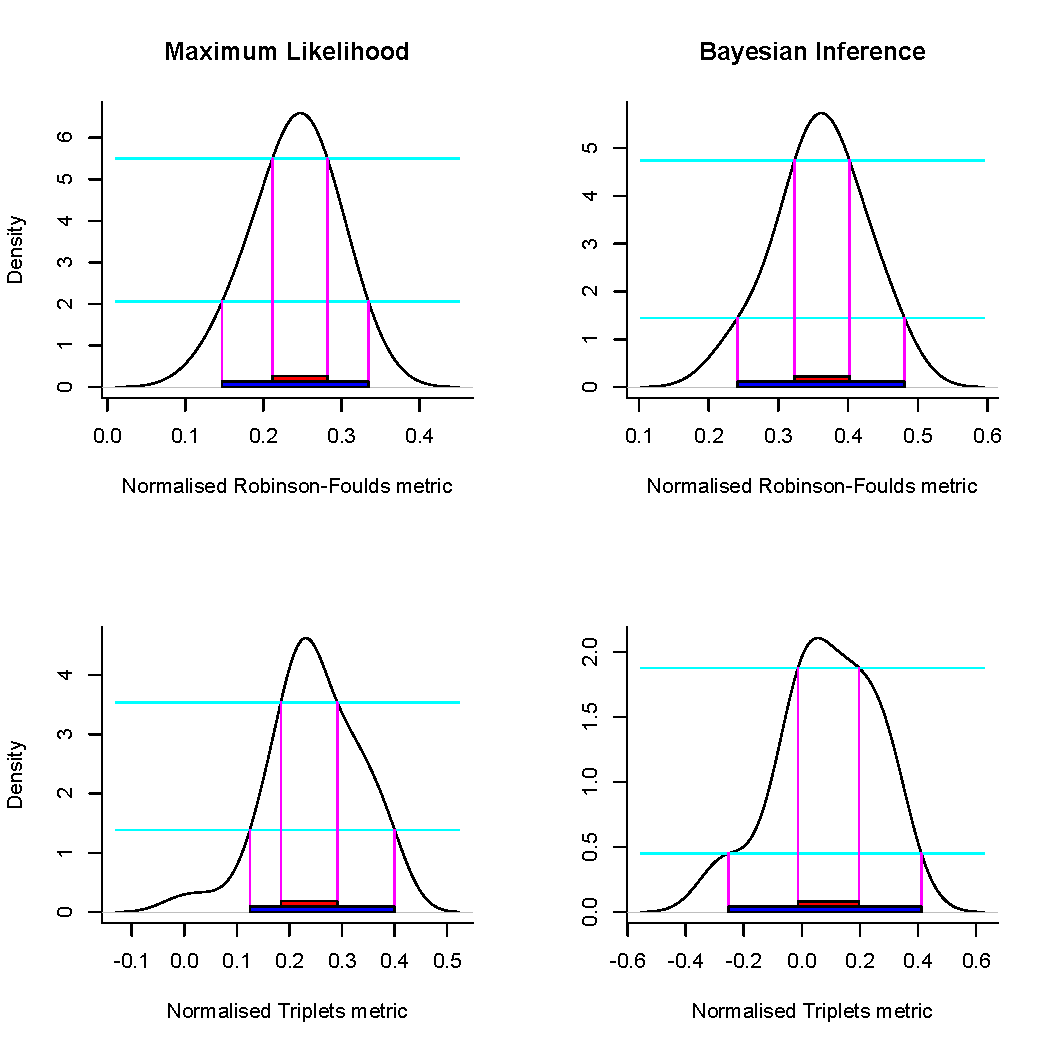
\includegraphics[width=1\textwidth]{SupplementaryFigures/True_vs_Best_trees.pdf}
    \caption{Pairwise comparisons among the 50 ``true'' trees and the 50 ``best'' trees from the Maximum Likelihood and Bayesian inference methods. The horizontal blue and red lines represent, respectively, the 95\% and 50\% confidence intervals.} 
\label{Fig_Supp_True_Best} 
\end{figure}


\bibliographystyle{sysbio}
\bibliography{Supp_Ref}

%END
\end{document}